\immediate\write18{tex celtic.dtx}
\documentclass{article}
\usepackage{tikz}
\usetikzlibrary{celtic}

\begin{document}

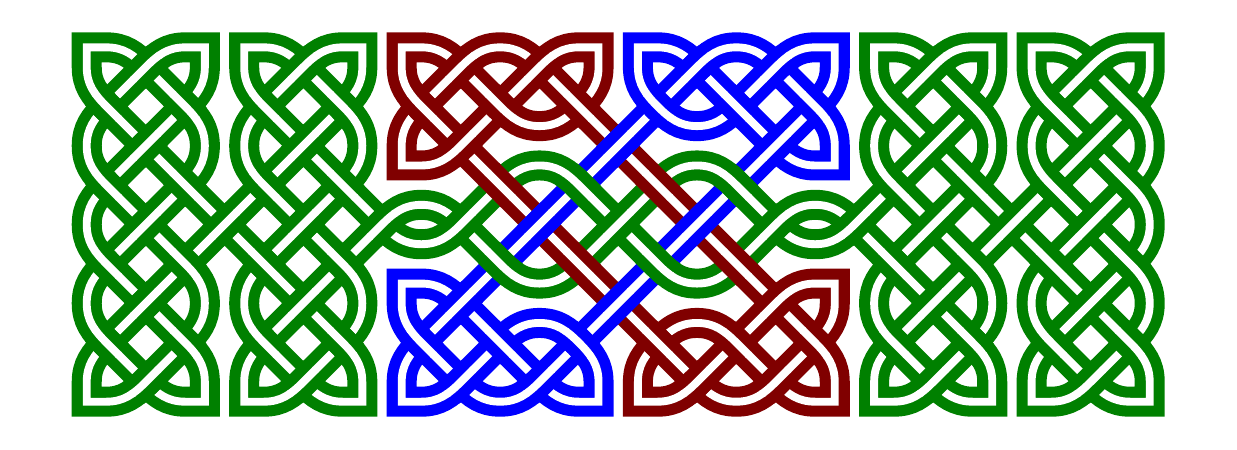
\begin{tikzpicture}[
  scale=.5,
  celtic path/.style={
    draw,
    double=white,%gray!40,
    red,
    double distance=1mm,
    line width=4pt
  },
  celtic path 1/.style={
    green!50!black,
  },
  celtic path 2/.style={
    blue,
  },
  celtic path 3/.style={
    red!50!black,
  },
  celtic surround/.style={
    ultra thick,
%    black,
%    fill=gray!40
  },
]
\CelticDrawPath{
  symmetric crossings={
    8,1:3,|;
    14,1,|;
    9,4,-;
    12,3,-;
    4,1,|;
    4,3,|;
%    10,5,-;
  },
  size={28,10},
  max steps=70
}
\path (current bounding box.west) +(-1,0);
\path (current bounding box.east) +(1,0);
\end{tikzpicture}
%\end{document}


\begin{tikzpicture}[
  scale=.5,
  celtic path/.style={
    draw,
    double=gray!40,
    red,
    double distance=1mm,
    line width=4pt
  },
  celtic path 1/.style={
    green!50!black,
  },
  celtic path 2/.style={
    blue,
  },
  celtic path 3/.style={
    red!50!black,
  },
  celtic surround/.style={
    ultra thick,
    black,
%    fill=black
  },
]
\CelticDrawPath{
  symmetric crossings={
    1,2,-;
    2,1,|;
    4,3,-;
    3,4,|;
  },
  size={8,8},
}
\end{tikzpicture}




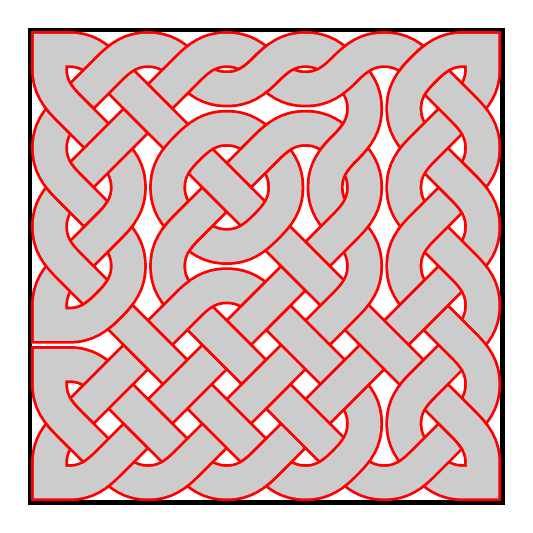
\begin{tikzpicture}[
  scale=.5,
  celtic path/.style={
    draw,
    double=gray!40,
    red,
    double distance=4mm,
    line width=1pt
  },
  celtic path 1/.style={
%    green
  },
  celtic path 2/.style={
%    blue
  },
  celtic surround/.style={
    ultra thick,
    black,
    draw
  },
]
\CelticDrawPath{
  size={12,12},
  crossings={
    5,6,-;
    3,8,|;
    7,8,|;
    5,10,-;
    7,10,-;
    3,6,|;
    9,8,|;
    9,6,|;
    9,10,|;
    1,4,-;
    9,2,|;
  },
  max steps={25}
}
\end{tikzpicture}


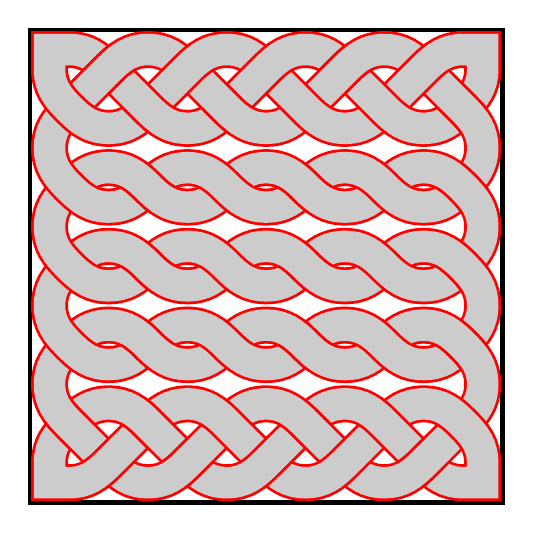
\begin{tikzpicture}[
  scale=.5,
  celtic path/.style={
    draw,
    double=gray!40,
    red,
    double distance=4mm,
    line width=1pt
  },
  celtic surround/.style={
    ultra thick,
    black,
    draw
  },
]
\CelticDrawPath{
  size={12,12},
  symmetric crossings={
    2:10,3:9,-
  },
  at={(1,1)}
}
\end{tikzpicture}

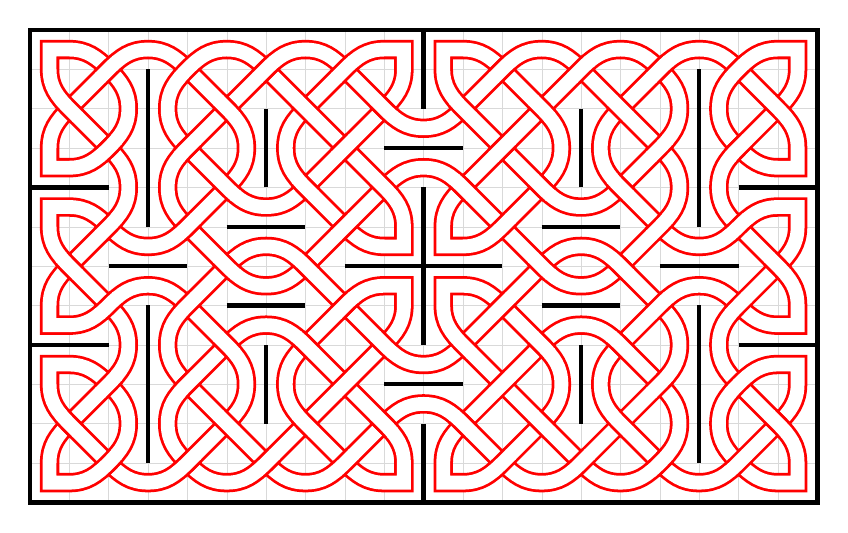
\begin{tikzpicture}[
  scale=.5,
  celtic path/.style={
    draw,
    double=white,
    red,
    double distance=5pt,
    line width=1pt
  },
  celtic bar/.style={
    ultra thick,
    black,
    draw
  },
]
\draw[gray!30,ultra thin] (0,0) grid (20,12);
\CelticDrawPath{
  size={20,12},
  symmetric crossings={
    10,1,|;
    3,2,|;
    3,4,|;
    6,3,|;
    10,5,|;
    10,3,-;
    9,6,-;
    6,5,-;
    3,6,-;
    1,4,-
  },
}
\end{tikzpicture}

\newpage

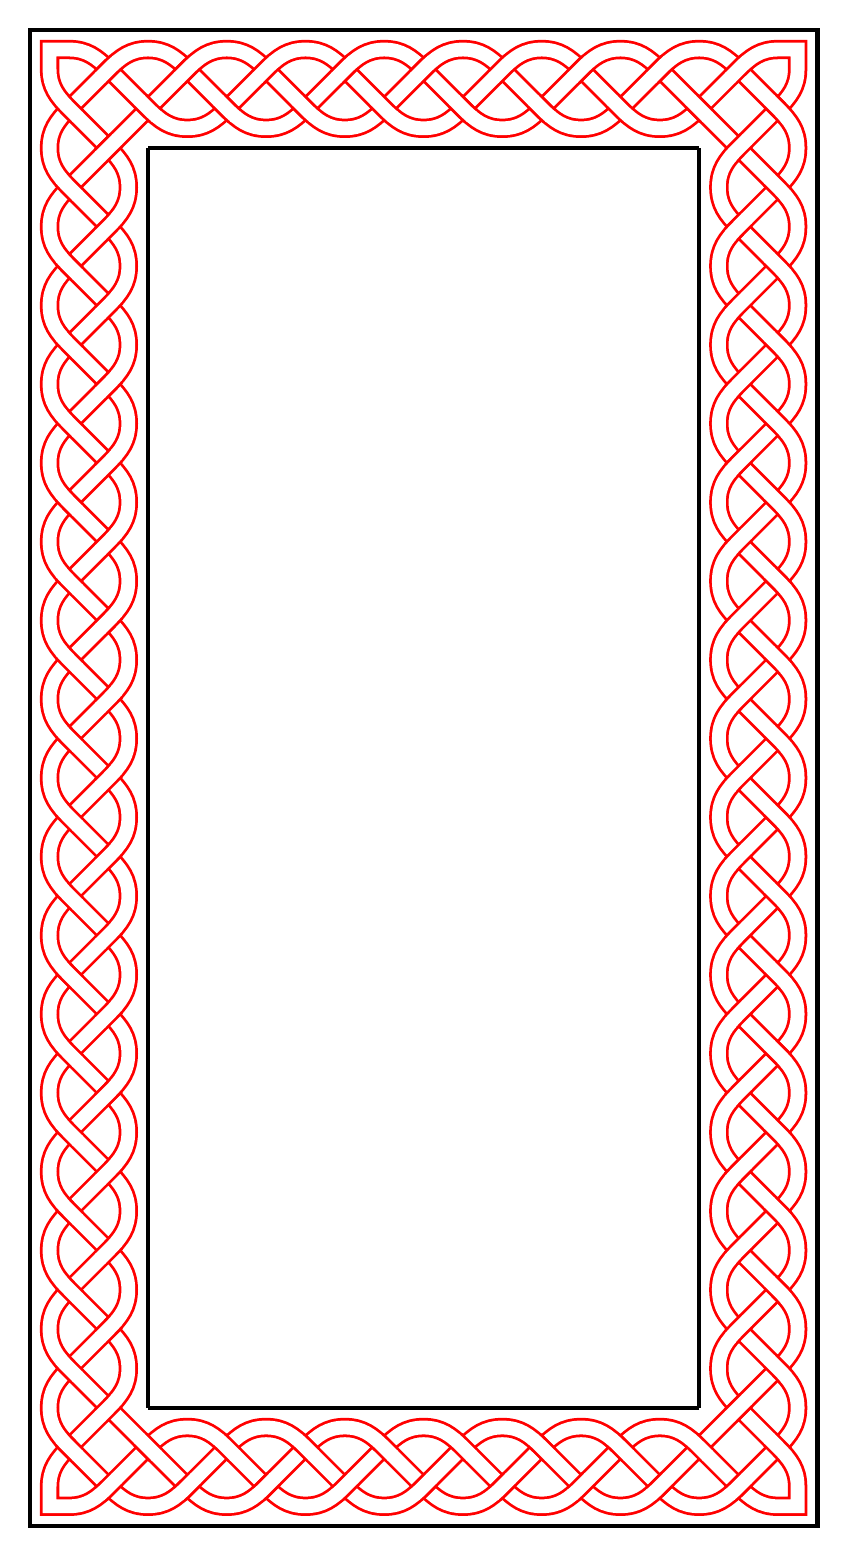
\begin{tikzpicture}[
  scale=.5,
  celtic path/.style={
    draw,
    double=white,
    red,
    double distance=5pt,
    line width=1pt
  },
  celtic bar/.style={
    ultra thick,
    black,
    draw
  },
]
\CelticDrawPath{
  size={20,38},
  symmetric crossings={
    3,4:34,|;
    4:16,3,-
  },
  ignore symmetric crossings={
    4:10,5:20;
    5:10,4:20
  },
  max steps=1000
}
\end{tikzpicture}



\end{document}

% Local Variables:
% tex-output-type: "pdf18"
% End:
